\usetikzlibrary{arrows.meta,calc}
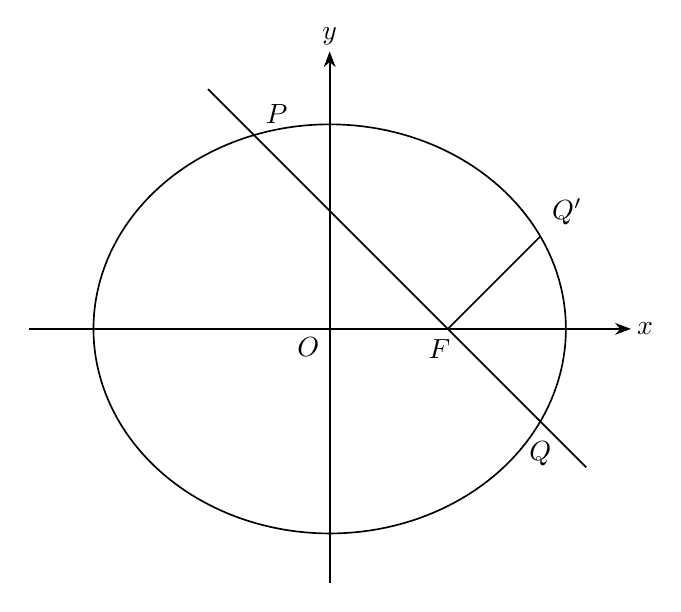
\begin{tikzpicture}[x=1.5cm,y=1.5cm,line width=.6pt,font=\normalsize,>=Stealth]
\def\ellA{2}
\def\ellB{1.7320508}
\coordinate (O) at (0,0);
\coordinate (F) at (1,0);
\coordinate (P) at (-0.6407545,1.6407545);
\coordinate (Q) at (1.7836116,-0.7836116);
\coordinate (Qp) at (1.7836116,0.7836116);
\coordinate (Lp) at (-1.0296632,2.0296632);
\coordinate (Lq) at (2.1725203,-1.1725203);
\draw[->] (-2.55,0)--(2.55,0) node[right,inner sep=0pt,xshift=2pt] {$x$};
\draw[->] (0,-2.15)--(0,2.35) node[above,inner sep=0pt,yshift=2pt] {$y$};
\draw plot[domain=0:360,samples=181,variable=\t] ({\ellA*cos(\t)},{\ellB*sin(\t)});
\draw (Lp)--(Lq);
\draw (F)--(Qp);
\node[above right,inner sep=4pt] at (P) {$P$};
\node[below=6pt,inner sep=1pt] at (Q) {$Q$};
\node[above right,inner sep=4pt] at (Qp) {$Q'$};
\node[anchor=center,inner sep=0pt] at (0.93,-0.17) {$F$};
\node[anchor=center,inner sep=0pt] at (-0.18,-0.15) {$O$};
\end{tikzpicture}
